% --------------------------------------------------------------------------------------------------
% Section: Results
% --------------------------------------------------------------------------------------------------

% Main section for presenting experiment outcomes
\section{Results} 

% --------------------------------------------------------------------------------------------------
% Subsection: Training Time and Performance
% --------------------------------------------------------------------------------------------------

\subsection{Training Time and Performance} 

% Description of training setup: model, hardware, and environment
The lung cancer detection model, based on the ResNet50 architecture, was trained on a labeled 
dataset of medical lung images. The training process was conducted using two different hardware 
configurations: a GPU-enabled environment and a traditional CPU-based environment.

% Table to present training metrics, [H] forces it to appear 'Here' (float package required)
\begin{table}[H]
\centering
\begin{tabular}{|c|c|c|}
    \hline
    \textbf{Hardware} & \textbf{Total Training Time} & \textbf{Average Time/Epoch} \\ 
    \hline
    \multicolumn{1}{|l|}{CPU (Apple M2, 10 cores)} & 
    \multicolumn{1}{l|}{5 hours 20 minutes} & 
    \multicolumn{1}{l|}{12.8 minutes} \\
    \hline
    \multicolumn{1}{|l|}{GPU (MPS)} & 
    \multicolumn{1}{l|}{48 minutes} & 
    \multicolumn{1}{l|}{1.92 minutes} \\
    \hline
\end{tabular}
\caption{Training Time Comparison over 20 Epochs}
\end{table}


% Explanation about CPU performance limitations for training deep models
While the CPU successfully completed the training task, it required several hours due to the 
computational intensity of deep convolutional neural networks like ResNet50. This highlights the 
limitations of using CPUs for large-scale deep learning tasks, particularly in terms of training 
time. The GPU significantly outperforms the CPU in terms of training time. This speedup allows for 
faster experimentation and model iteration.

% Figure comparing training times
\vspace{1em}
\begin{center} 
    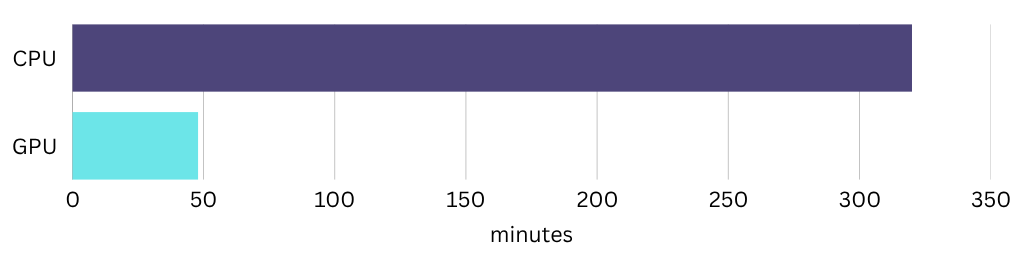
\includegraphics[width=\textwidth]{../assets/07-results/graph-cpu-vs-gpu.png} 

    \small\textit{Chart comparison of training time between GPU and CPU.} 
\end{center}
\vspace{1em} 

% --------------------------------------------------------------------------------------------------
% Subsection: Energy and CO2 Footprint Analysis
% --------------------------------------------------------------------------------------------------

\subsection{Energy and CO\textsubscript{2} Footprint Analysis}

To further understand the environmental and economic implications, we compared the energy 
consumption and estimated CO\textsubscript{2} emissions of the two setups.

\begin{table}[H]
\centering
\begin{tabular}{|c|c|c|c|c|}
    \hline
    \textbf{Hardware} & \textbf{Power Usage} & \textbf{Time} & \textbf{Energy} & 
    \textbf{CO\textsubscript{2} Emission (kg)} \\
    \hline
    \multicolumn{1}{|l|}{CPU} & 
    \multicolumn{1}{l|}{65 W} & 
    \multicolumn{1}{l|}{5.33 h} & 
    \multicolumn{1}{l|}{0.346} & 
    \multicolumn{1}{l|}{$\approx$0.277} \\
    \hline
    \multicolumn{1}{|l|}{GPU} & 
    \multicolumn{1}{l|}{320 W} & 
    \multicolumn{1}{l|}{0.8 h} & 
    \multicolumn{1}{l|}{0.256} & 
    \multicolumn{1}{l|}{$\approx$0.205} \\
    \hline
\end{tabular}
\caption{Energy Consumption and CO\textsubscript{2} Emission Estimates}
\end{table}

\newpage

Assumptions:
\begin{itemize}
    \item CO\textsubscript{2} emission factor: 0.8 kg CO\textsubscript{2} per kWh 
    (based on global average).
    \item Electricity cost: \$0.15 per kWh (average in the US).
\end{itemize}

% --------------------------------------------------------------------------------------------------
% Subsection: Cost Calculation
% --------------------------------------------------------------------------------------------------

\subsection{Cost Calculation}

\begin{itemize}
    \item \textbf{CPU Total Cost} = 0.346 kWh $\times$ \$0.15 = \textbf{\$0.0519}
    \item \textbf{GPU Total Cost} = 0.256 kWh $\times$ \$0.15 = \textbf{\$0.0384}
\end{itemize}

% --------------------------------------------------------------------------------------------------
% Subsection: Theoretical GPU Performance (Compared to CPU)
% --------------------------------------------------------------------------------------------------

\subsection{Theoretical GPU Performance (Compared to CPU)}

% Discussion of GPU strengths for deep learning tasks
Although the training was conducted on a CPU, it is important to consider the theoretical 
performance advantages of GPUs. Graphics Processing Units (GPUs) are highly optimized for parallel 
floating-point computations, which are common in deep learning tasks. The performance of GPUs is 
often measured in TFLOPS (Tera Floating Point Operations Per Second).

% --------------------------------------------------------------------------------------------------
% Subsubsection: Effective TFLOPS Calculation
% --------------------------------------------------------------------------------------------------

% Unnumbered subsubsection for showing the formula
\subsubsection*{Effective TFLOPS Calculation} 

% Formula for calculating FLOPS
\[
\text{FLOPS} = \text{Number of Cores} \times \text{Clock Speed (Hz)} \times \text{FLOPs per Cycle}
\]

% Conversion from FLOPS to TFLOPS
\[
\text{TFLOPS} = \frac{\text{FLOPS}}{10^{12}}
\]

% Example calculation using GPU specs
For example, a GPU with:
\begin{itemize}
    \item 8704 MPS cores
    \item Clock speed of 1.7 GHz
    \item 2 FLOPs per core per cycle
\end{itemize}

would yield:

% FLOPS calculation with example values
\[
\text{FLOPS} = 8704 \times 1.7 \times 10^9 \times 2 = 29.6 \times 10^{12} = 29.6 \text{ TFLOPS}
\]

% Note on how this compares to CPU performance
This is several orders of magnitude higher than a standard CPU, which may reach only up to 0.5–1.5 
TFLOPS under optimal conditions.

% TFLOPS comparison image
\vspace{1em} 
\begin{center} 
    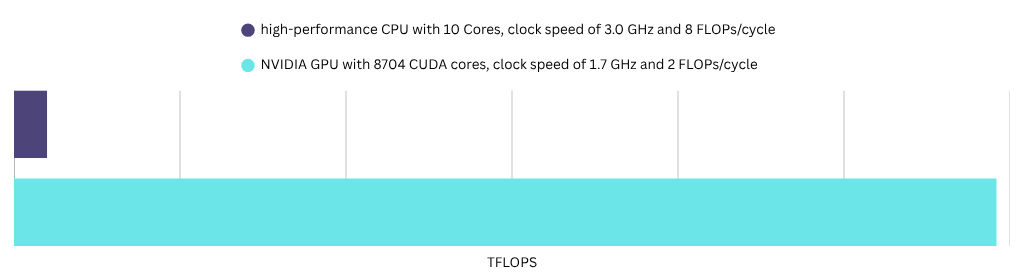
\includegraphics[width=\textwidth]{../assets/07-results/tflops-cpu-vs-gpu.png} 
    \small\textit{Chart comparison of TFLOPS values between GPU and CPU.} 
\end{center}
\vspace{1em} 

% --------------------------------------------------------------------------------------------------
% Subsection: Components Influencing Training Speed
% --------------------------------------------------------------------------------------------------

\subsection{Components Influencing Training Speed}

% List of hardware/software factors that affect model training speed
Several hardware and software factors significantly influence deep learning training performance:

\begin{itemize}
    % Critical for speeding up tensor operations
    \item \textbf{Core Count and Parallelism} – More cores allow parallel execution of matrix 
    operations. 

    % Affects throughput but with trade-offs
    \item \textbf{Clock Speed} – Higher frequencies can increase operation speed, but also power 
    consumption. 

    % Prevents memory bottlenecks
    \item \textbf{Memory Bandwidth} – High-speed memory access is critical for transferring large 
    tensors during training. 

    % Important for temporal locality of data
    \item \textbf{Cache Size and Architecture} – Affects the ability to reuse data without frequent 
    memory access. 

    % Code-level tuning makes majorimpact
    \item \textbf{Software Optimization} – Efficient usage of libraries such as PyTorch with 
    multithreading and vectorization can impact performance greatly. 
\end{itemize}

% --------------------------------------------------------------------------------------------------
% Subsection: Summary of GPU vs CPU Comparison
% --------------------------------------------------------------------------------------------------

\subsection{Summary of GPU vs CPU Comparison}

\begin{itemize}
    \item \textbf{Training Speed:} GPU offers a 6.7x speed improvement over CPU.
    \item \textbf{Energy Efficiency:} Despite higher power usage, GPU finishes faster, leading to 
    lower overall energy consumption.
    \item \textbf{Cost-Effective:} GPU-based training costs less in terms of energy bills.
    \item \textbf{CO\textsubscript{2} Emissions:} GPU results in a slightly lower carbon footprint.
\end{itemize}